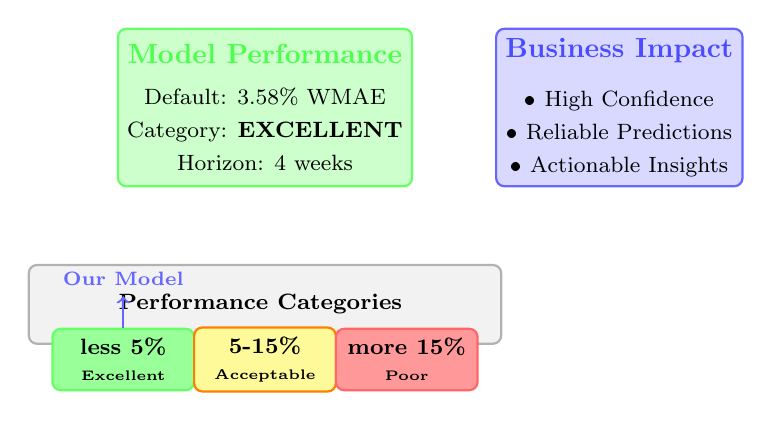
\begin{tikzpicture}[
	box/.style={rectangle, rounded corners=3pt, draw, thick, align=center},
	main/.style={box, fill=green!20, draw=green!60, minimum width=3.5cm, minimum height=2cm},
	scalebox/.style={box, fill=gray!10, draw=gray!60, minimum width=6cm, minimum height=1cm},
	cat/.style={box, minimum width=1.8cm, minimum height=0.7cm, font=\footnotesize\bfseries},
	impact/.style={box, fill=blue!15, draw=blue!60, minimum width=2.8cm, minimum height=2cm}
	]
	
	% Main performance box
	\node[main] (perf) at (0,0) {
		\textbf{\color{green!70}Model Performance}\\[0.1cm]
		\footnotesize Default: 3.58\% WMAE\\
		\footnotesize Category: \textbf{EXCELLENT}\\
		\footnotesize Horizon: 4 weeks
	};
	
	% Performance scale container
	\node[scalebox] (scale) at (0,-2.5) {
		\textbf{\footnotesize Performance Categories}
	};
	
	% Category boxes positioned within scale
	\node[cat, fill=green!40, draw=green!60] (exc) at (-1.8,-3.2) {less 5\%\\{\tiny Excellent}};
	\node[cat, fill=yellow!40, draw=orange] (acc) at (0,-3.2) {5-15\%\\{\tiny Acceptable}};
	\node[cat, fill=red!40, draw=red!60] (poor) at (1.8,-3.2) { more 15\%\\{\tiny Poor}};
	
	% Arrow pointing to our category
	\draw[->, thick, blue!60] (exc.north) -- ++(0,0.4) node[above, font=\scriptsize\bfseries] {Our Model};
	
	% Business impact box
	\node[impact] (bus) at (4.5,0) {
		\textbf{\color{blue!70}Business Impact}\\[0.2cm]
		\footnotesize • High Confidence\\
		\footnotesize • Reliable Predictions\\
		\footnotesize • Actionable Insights
	};
	
\end{tikzpicture}